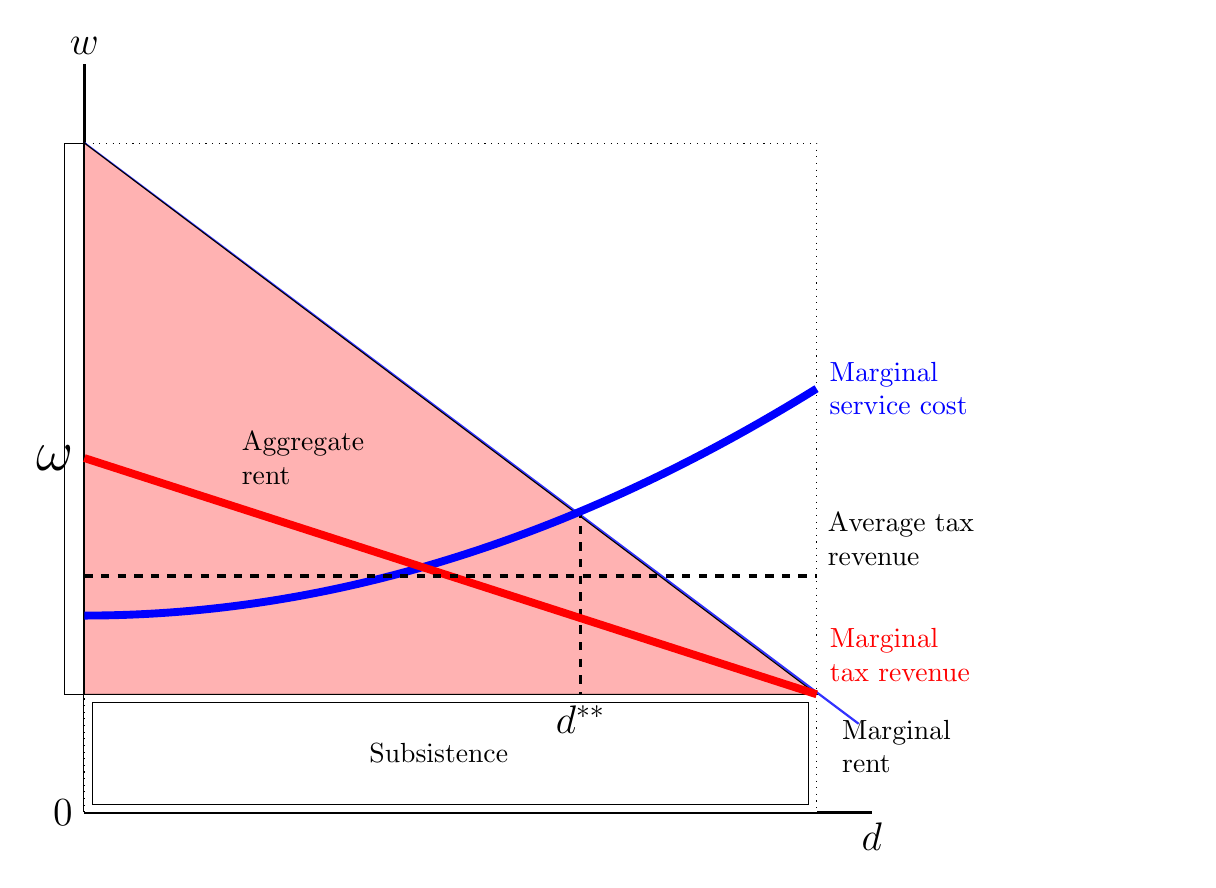
\begin{tikzpicture}[scale=1]
\def\bndmax{5}        %https://tex.stackexchange.com/questions/68462/filling-a-complex-region-with-tikz
\def\bndmin{0.2}
\def \n {8}  % height of y axis
\def \d {10}  % length  of x axis
\def \t {.75}  %  cost of transportation per unit x
\def \th {1}   %
\def \w {7}    %  wage premium
\def \om{1.5}%  omega =rural wage Zero for urban population
\def \azero{2}
\def \aprime {-.0}	
\tikzset{func/.style={thick,color=blue!80}}	
\draw [thick] (0,-\om) --(\d,-\om)node[below]{\Large $d$};  			% Zero for rural population
\draw [thick] (0,-\om)node[left=.5]{\Large $0$} --(0,\n)node[above]{\Large $w$};	% Y axis

%\draw [thick] (0,0)node[left=.5]{ subsistance}--(\d,0);
\node[left=.25] at (0,3){\huge $\omega$};
%\node[left=.25] at (0,\w+.3){subsistence plus};
%\node[left=.25] at (0,\w-.4){wage premium};	

\draw[fill=white, white] (0.1,-0.1) rectangle (14,-\om+.1);
\draw [] (-.25, 0) rectangle(.25, \w);%fill=green!30!blue!30
\node[right] at  (.25, \w/2){Added Productivity};
%\draw [ thick, ->](11.3,-\om/2)--(13, -\om/2)node [right] {\Large $d$};
\draw[fill=blue!40] (0.1,-0.1) rectangle (9.2,-\om+.1);

\draw[fill=black!0, dotted] (0,-\om) rectangle (9.30,\w);% new product repeat
\draw[func, domain=0:\w/\t+.5] plot [samples=200] (\x,{\w-\t*\x}); %rent profile
\draw[fill=blue!0] (0.1,-0.1) rectangle (9.2,-\om+.1);
\node at (4.5,-\om/2){Subsistence};
\draw[fill=red!30,] (0.,0.)--(0,7)--(9.30,0.)--cycle;% Rent \w-.2
\node[text width=2cm] at (3.,3){Aggregate \\rent}; 		%Rent 
%\node at (5.8,5.7)[]{\Large Transportation};
\node at (6.3,4.8)[white]{\Large expenditure};
\draw[ line width=.5mm, dashed] (6.3,2.35)--(6.3,0)node[below ]{\Large $d^{**}$};

\draw[func, domain=0:9.3, line width=1mm,blue, text width=2cm] plot [samples=200] (\x,{1+\x^2/30})node[right]{Marginal\\ service cost};
\draw[ line width=1mm, red] (0,3)--(9.3,0)node[above right, text width=3cm ]{Marginal\\tax revenue};
\node at (9.5, -.2)[below right, text width=2cm]{Marginal rent};

\draw[ line width=.5mm, dashed] (0,1.5)--(9.3,1.5)node[above right, text width=2.5cm ]{Average tax revenue};
%GRID
%\draw[step=1cm,gray,very thin] (0,0) grid (10,10);
\end{tikzpicture}